\documentclass[a4paper]{article}

%% Language and font encodings
\usepackage[english]{babel}
\usepackage[utf8]{inputenc}
\usepackage[T1]{fontenc}

%% Sets page size and margins
\usepackage[a4paper,top=3cm,bottom=2cm,left=3cm,right=3cm,marginparwidth=1.75cm]{geometry}

%% Useful packages
\usepackage{amsmath}
\usepackage{graphicx}
\usepackage[colorinlistoftodos]{todonotes}
\usepackage[colorlinks=true, allcolors=blue]{hyperref}
\usepackage{wrapfig}



%% Bibtex
\usepackage[backend=bibtex,style=ieee]{biblatex}


\usepackage{tikz} %Tikz !
\usetikzlibrary{arrows,automata,calc}

\usepackage{listings}
\usepackage{color}

\definecolor{darkWhite}{rgb}{0.94,0.94,0.94}
\lstset{
	aboveskip=3mm,
	belowskip=-2mm,
	backgroundcolor=\color{darkWhite},
	basicstyle=\footnotesize,
	breakatwhitespace=false,
	breaklines=true,
	captionpos=b,
	commentstyle=\color{red},
	deletekeywords={...},
	escapeinside={\%*}{*)},
	extendedchars=true,
	framexleftmargin=16pt,
	framextopmargin=3pt,
	framexbottommargin=6pt,
	frame=tb,
	keepspaces=true,
	keywordstyle=\color{blue},
	language=C,
	literate=
	{²}{{\textsuperscript{2}}}1
	{⁴}{{\textsuperscript{4}}}1
	{⁶}{{\textsuperscript{6}}}1
	{⁸}{{\textsuperscript{8}}}1
	{€}{{\euro{}}}1
	{é}{{\'e}}1
	{è}{{\`{e}}}1
	{ê}{{\^{e}}}1
	{ë}{{\¨{e}}}1
	{É}{{\'{E}}}1
	{Ê}{{\^{E}}}1
	{û}{{\^{u}}}1
	{ù}{{\`{u}}}1
	{â}{{\^{a}}}1
	{à}{{\`{a}}}1
	{á}{{\'{a}}}1
	{ã}{{\~{a}}}1
	{Á}{{\'{A}}}1
	{Â}{{\^{A}}}1
	{Ã}{{\~{A}}}1
	{ç}{{\c{c}}}1
	{Ç}{{\c{C}}}1
	{õ}{{\~{o}}}1
	{ó}{{\'{o}}}1
	{ô}{{\^{o}}}1
	{Õ}{{\~{O}}}1
	{Ó}{{\'{O}}}1
	{Ô}{{\^{O}}}1
	{î}{{\^{i}}}1
	{Î}{{\^{I}}}1
	{í}{{\'{i}}}1
	{Í}{{\~{Í}}}1,
	morekeywords={*,...},
	numbers=left,
	numbersep=10pt,
	numberstyle=\tiny\color{black},
	rulecolor=\color{black},
	showspaces=false,
	showstringspaces=false,
	showtabs=false,
	stepnumber=1,
	stringstyle=\color{gray},
	tabsize=4,
	title=\lstname,
}
\hypersetup{
	urlcolor= blue,  %couleur des hyperliens
	linkcolor= black, %couleur des liens internes
}

\bibliography{bib/kilobots} 
%%\nocite{*} %% A CHANGER POUR LES CITATIONS : exemple Je cite \cite{nom_article}
\newcommand{\HRule}{\rule{\linewidth}{0.5mm}} % Defines a new command for the horizontal lines, change thickness here



\title{Robotique en essaim}
\author{Andres Julien, Taylor Thomas}
\date{}
\begin{document}

\begin{titlepage}
\center
\includegraphics{incl/logo_sorbonne}\\[1cm] 

\HRule \\[0.4cm]
{ \huge \bfseries Robotique en essaim}\\[0.4cm] % Title of your document
\HRule \\[1.5cm]



Julien \textsc{Andres}\\ % Your name
Thomas \textsc{Taylor}\\[3cm]
Nicolas \textsc{Bredeche}\\[3cm]


\includegraphics[width=4cm]{incl/Kilobots.png}



\end{titlepage}

\newpage
\renewcommand{\contentsname}{Sommaire}
\tableofcontents
\newpage
\section{Introduction}
\subsection{Robotique en essaim}
La robotique en essaim s'inspire d'observations d'insectes et d'animaux sociaux pour l'étude de comportements collectifs issus de simples tâches individuelles. Les principales propriétés de ce domaine sont la robustesse, grâce à un code décentralisé, et l'échelle proposée, le code pouvant être déployé sur différentes tailles d'essaim.
\subsection{Couverture}
La couverture est un problème fondamental dans la robotique en essaim. En effet, elle permet aux robots de se déployer dans un environnement inconnu ou dynamiques, tout en maintenant un contact entre eux. Ce problème se retrouve dans beaucoup de domaine, comme le sauvetage de personnes en milieu hostile ou inconnu.
\subsection{Agrégation}
L'agrégation est un comportement de base des essaims. Il permet aux organismes de faire face ensemble à un problème. Dans le domaine de la robotique en essaim, ce comportement permet a des robots dispersés dans un environnement de se regrouper en un ou plusieurs groupes.
\subsection{Algorithmes génétiques en ligne}
L'objectif de ces algorithmes est d'arriver, à partir d'un génome aléatoire définissant un comportement d'un robot, à un comportement permettant au robot de survivre dans son environnement. L'aspect \textit{en-ligne} de l'algorithme représente la distribution du code sur l'ensemble des robots. ??? ajouter apprentissage ensemble ??
\subsection{Problématique}
L'objectif de ce projet est de tester le dispositif expérimental en implémentant des comportements simples d'agrégation et de couverture ainsi qu'un comportement plus évolué d'agrégation. \\Dans un second temps, nous étudierons un algorithme dit d'\textit{embodied evolution}, ce type d'algorithme distribué est plus léger et permet de converger vers des comportements opérant un compromis entre survie (proximité d'un point de recharge) et diffusion du jeu de paramètres (permettant à l'essaim une plus grande chance de survie collective)
\newpage
\section{Matériel utilisé}
\subsection{Kilobot}
Un Kilobot \cite{rubenstein_kilobot:_2012} est un robot miniature, créé par l'université d'Harvard. Ces robots permettent l'étude de la robotique en essaim, leur faible cout étant un avantage pour la manipulation d'un grand nombre d'individus.
\paragraph{Communication}Les robots peuvent communiquer entre eux grâce à des messages qu'ils envoient à leurs voisins à une distance d'environ 7cm. L'intensité du signal permet à un Kilobot d'évaluer la distance à laquelle se trouve la source du message. Chaque robot possède aussi un capteur de luminosité.
\paragraph{Mouvements}Chaque robot possède deux moteurs, placé de chaque coté de son corps. Ils permettent au robot d'avancer en faisant vibrer ses pattes. Les déplacement d'un Kilobot se font donc en modulant la vitesse de chacun de ses moteurs selon la direction voulu.\\
\begin{figure}[h]
	\begin{center}
		\centering
		\includegraphics[width=0.8\linewidth]{incl/kilobot-closeup-overview.jpg}
		\caption{Kilobot}
	\end{center}
\end{figure} \\
Les comportements des robots sont écrits en C, en utilisant l'API kilolib et peut être transmis à l'ensemble des Kilobots  grâce à un contrôleur infrarouge.
reçoit
\subsection{Bloc Actif}
Le bloc actif a été développé par l'ISIR dans le cadre de la recherche sur Kilobots. Elle permet d'interagir avec les robots en émettant un signal infrarouge. Le numéro du message et l'intensité du signal peuvent être modulé grâce à des boutons sur le bloc actif. Il fera office d'obstacle et de point de ralliement pour certains de nos algorithmes.\\
\begin{figure}[h]
	\begin{minipage}[c]{.46\linewidth}
		\centering
		\includegraphics[width=1.1\linewidth]{../../script_results/bloc_actif_max.jpg}
		\caption{Distance max à intensité max}
	\end{minipage}
	\hfill%
	\begin{minipage}[c]{.46\linewidth}
		\centering
		\includegraphics[width=1.1\linewidth]{../../script_results/bloc_actif_min.jpg}
		\caption{Distance max à intensité min}
	\end{minipage}
\end{figure}
\\
Les robots devant êtres vraiment trop collés au bloc pour recevoir le signal en intensité minimale, nous utiliserons dans toutes les expériences l'intensité maximale du bloc actif.
\subsection{Arène}
Les algorithmes ont été testé sur un essaim de 70 robots, fournit par le laboratoire de rechercher ISIR. L'arène utilisé pour l'étude des algorithme faisait 1x1.5 mètres.\\
\begin{figure}[h]
	\begin{center}
		\centering
		\includegraphics[scale=0.4,angle=-90]{../../script_results/arene.png}
		\caption{Modélisation  d'un gradient sur simulateur}
	\end{center}
\end{figure} \\

\subsection{Simulateur}
Afin de faciliter le développement et l'étude des algorithmes, le simulateur Kilombo \cite{jansson_kilombo:_2015} a été utilisé. Il inclut l'API kilolib et permet ainsi une compatibilité direct du code entre le simulateur et l'essaim de robots.
\begin{figure}[h!]
	\begin{center}
		\centering
		\includegraphics[width=0.8\linewidth]{../../script_results/gradient2-sim.png}
		\caption{Modélisation  d'un gradient sur simulateur}
	\end{center}
\end{figure} 
\newpage
\section{Couverture}
\subsection{Algorithme}
Cet algorithme est utilisé afin de couvrir la plus grande surface possible, tout en gardant un lien de communication entre les Kilobots.
Il est composé de 3 comportements basique : L'éloignement (\textit{repel}), le déplacement aléatoire(\textit{searching}) et l'attente(\textit{wait})
\paragraph{Le déplacement aléatoire} Ce comportement s'effectue lorsque le Kilobot ne détecte aucun voisin. Il bouge alors aléatoirement dans son environnement jusqu'à la détection d'un autre robot. Il passe alors en mode d'attente ou d'éloignement selon la distance à laquelle il est de ses voisins.
\paragraph{L'éloignement} Si le Kilobot se trouve trop proche de ses voisins, il essayera de s'en éloigner. Soit en s'éloignant de son voisin le plus proche, soit en bougeant aléatoirement jusqu'à être à une distance désiré de tous ses voisins.
\paragraph{L'attente} Le Kilobot entre en attente quand il se trouve à une distance supérieure ou égale à celle demandé de tous ses voisins. Il sort de ce comportement s'il ne capte plus aucun voisins ou si un Kilobot arrive trop proche.\\


\begin{figure}[h!]
\centering
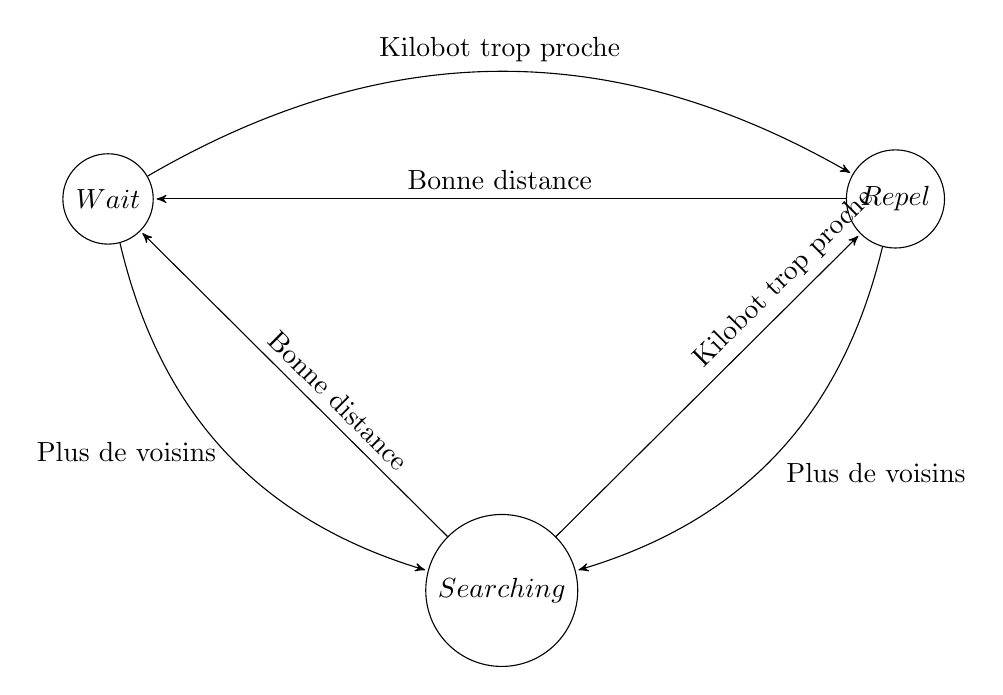
\begin{tikzpicture}[>=stealth',shorten >=1pt,auto,node distance=10cm]
\node[state] (W)      {$Wait$};
\node[state] (R) [right of=W]  {$Repel$};
\node[state] at ($(W)!0.5!(R)$) [below =4cm] (S)  {$Searching$};


\path[->]
(W) edge  [bend left,sloped] node {Kilobot trop proche} (R)
(R) edge   [sloped]node {Bonne distance} (W)
(W) edge   [bend right,anchor=east]node {Plus de voisins} (S)
(S) edge   [sloped,pos=0.4,align=right,anchor=south]node {Bonne distance} (W)
(R) edge   [bend left]node {Plus de voisins} (S)
(S) edge   [sloped,pos=0.8]node {Kilobot trop proche} (R);
\end{tikzpicture}
\caption{Couverture}
\end{figure}
\newpage
\subsection{Résultats}
Deux positions de départ sont possible pour l'essaim de Kilobot pour le problème de couverture. Nous pouvons partir d'un essaim regroupé en un groupe compact ou d'un essaim éparpillé sur l'ensemble de l'environnement.
Nous étudions ici le comportement de l'essaim en fonction de la distance minimale demandé entre chaque robot.


\begin{figure}[h]
	\begin{minipage}[c]{.46\linewidth}
		\centering
		\includegraphics[width=1.1\linewidth]{../../script_results/start_groupe_real.png}
		\caption{Commencement groupé}
	\end{minipage}
	\hfill%
	\begin{minipage}[c]{.46\linewidth}
		\centering
		\includegraphics[width=1.1\linewidth]{../../script_results/start_eparpille_real.png}
		\caption{Commencement éparpillé}
	\end{minipage}
\end{figure}



\subsubsection{Commencement groupé}

\begin{figure}[h]
	\begin{minipage}[c]{.46\linewidth}
		\centering
		\includegraphics[width=1.1\linewidth]{../../script_results/Couverture_taille_cluster_groupe.png}
		\caption{Nombre de cluster selon la distance}
	\end{minipage}
	\hfill%
	\begin{minipage}[c]{.46\linewidth}
		\centering
		\includegraphics[width=1.1\linewidth]{../../script_results/Couverture_average_robot_groupe.png}
		\caption{Taille moyenne d'un cluster selon la distance}
	\end{minipage}
\end{figure}
\begin{figure}[h!]
	\centering
	\begin{minipage}[c]{.46\linewidth}
		\centering
		\includegraphics[width=1.1\linewidth]{../../script_results/Couverture_loss_kilobot_groupe.png}
		\caption{Nombre de Kilobot perdu selon la distance}
	\end{minipage}
\end{figure}
On remarque ici un nombre très bas de robot \textit{perdus} (c'est a dire qui n'appartiennent à aucun groupe). \\Le nombre de robots dans un agrégat (c'est à dire un groupe de Kilobot en attente, communiquant tous ensemble) est assez grand pour des valeurs inférieures à 55mm, ce qui s'explique par la proximité des robots dés le départ. Les robots étant proches, il est normal qu'ils soient bien connectés entre eux.
\subsubsection{Commencement éparpillé}
\begin{figure}[h]
	\begin{minipage}[c]{.46\linewidth}
		\centering
		\includegraphics[width=1.1\linewidth]{../../script_results/Couverture_average_robot.png}
		\caption{Nombre de cluster selon la distance}
	\end{minipage}
	\hfill%
	\begin{minipage}[c]{.46\linewidth}
		\centering
		\includegraphics[width=1.1\linewidth]{../../script_results/Couverture_taille_cluster.png}
		\caption{Taille moyenne d'un cluster selon la distance}
	\end{minipage}
\end{figure}
On remarque immédiatement que plus la distance entre deux robot est grande (elle ne dépasse jamais la distance maximale de communication), moins la couverture est efficace. On remarque que plus la distance demandé est grande, plus le nombre total de groupe est grand et plus leur taille est petite. En effet, le groupe de robot, cherchant à atteindre cette distance minimale, va se fractionner et de nombreux petits groupes se formeront. 

\begin{figure}[h!]
	\begin{minipage}[c]{.46\linewidth}
		\centering
	\includegraphics[width=1.1\linewidth]{../../script_results/Couverture_loss_kilobot.png}
	\caption{Nombre de Kilobot perdu selon la distance}
	\end{minipage}
	\begin{minipage}[c]{.46\linewidth}
	On remarque aussi, que plus la distance est grande, plus le nombre de Kilobot \textit{perdus} est grand. On observe un grand grand changement entre une distance de 60 et de 65. Ce grand écart est aussi observable sur les graphiques précédents.
	\end{minipage}
\end{figure}
\newpage
\subsubsection{Comparaison}
On remarque que le départ depuis un essaim groupé amène à une configuration des Kilobots plus connectés contenant moins de robots perdus qu'un départ éparpillé.En effet, la proximité des Kilobots dés le début de l'expérience les empêche de rester seul.\\ Cependant, cette connexité se fait au détriment de la durée de convergence de l'algorithme, qui est plus rapide depuis un essaim éparpillé (l'aléatoire ayant déjà fait une partie du travail).
\newpage
\section{Agrégation}
\subsection{Agrégation naïve}
Le but de cet algorithme est de faire s'agréger les Kilobot vers un objet  pouvant représenter une source de nourriture par exemple. Cet objet sera représenté ici par le bloc actif. Le principal but de cet algorithme étant de former un groupe compact de Kilobot, autour du bloc actif.\\
Dans cet algorithme, les robots ne communique que pour indiquer l'emplacement du bloc actif. Ils n'ont donc aucune autre information sur leur environnement. Cet algorithme est composé de 3 comportements : la recherche, l'approche et l'émission.\\
\paragraph{Recherche} Le robot bouge aléatoirement dans son environnement afin de trouver une source d'émission. Ici, le Kilobot ne fait aucune hypothèse sur son environnement. Il n'émet rien et ne reçoit donc aucune information provenant des autres robots dans le même état que lui. Ce comportement cesse lorsqu'il reçoit un message, le prévenant de la présence du bloc actif ou d'un robot proche de ce bloc actif. Il passe alors en comportement d'approche.
\paragraph{L'approche} Lors de cette phase, le robot va essayer de s'approcher du signal le plus proche. La méthode d'approche utilisé (qui est la même dans tous les algorithmes qui suivent) consiste à approcher en faisant des rotations. A la réception du message, le robot choisit aléatoirement une direction entre droite et gauche. A chaque nouveau message, si le Kilobot s'est rapproché de la source, il continue dans la même direction, sinon il prend la direction opposé.\\Il sort de ce comportement s'il perd le signal de la source (retourne à la recherche) ou s'il est assez proche de tous ses voisins émetteurs. Il passe alors dans l'état d'émission.
\paragraph{Émission} Le robot se trouve à une distance inférieure ou égale à celle demandé par l'algorithme. Il se met donc à émettre a son tour afin de transmettre l'information aux robots qui lui sont proches.

\begin{figure}[h!]
	\centering
	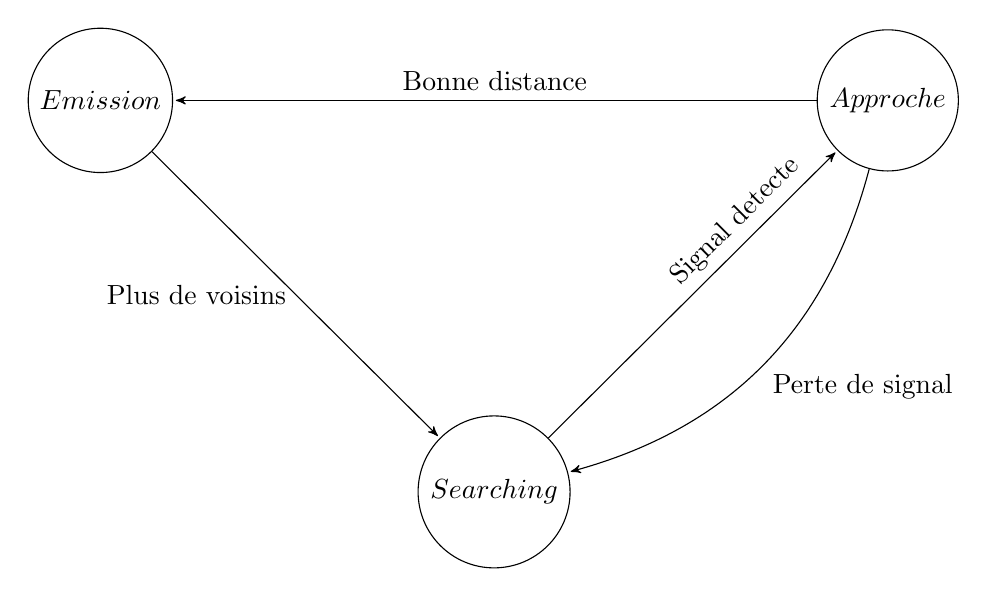
\begin{tikzpicture}[>=stealth',shorten >=1pt,auto,node distance=10cm]
	\node[state] (W)      {$Emission$};
	\node[state] (R) [right of=W]  {$Approche$};
	\node[state] at ($(W)!0.5!(R)$) [below =4cm] (S)  {$Searching$};
	
	
	\path[->]
	(R) edge   [sloped]node {Bonne distance} (W)
	(W) edge   [anchor=east]node {Plus de voisins} (S)
	(R) edge   [bend left]node {Perte de signal} (S)
	(S) edge   [sloped,pos=0.7]node {Signal detecte} (R);
	\end{tikzpicture}
	\caption{Agrégation Naïve}
\end{figure}
\newpage
\subsection{Agrégation probabiliste}

Cet algorithme découle de celui présenté par O.Soysal et E.Sahin. \cite{soysal_probabilistic_2005} Il permet aux robots de s'agglomérer basé sur une probabilité calculé indépendamment par chaque robot.\\

Il est composé de 4 comportement basiques : l'approche
(\textit{approach}), l'attente
(\textit{wait}), l'éloignement 
(\textit{repel}) et un évitement d'obstacle.
Un Kilobot n'ayant pas de capteur de proximité, il lui est impossible de détecter un obstacle tel qu'un mur. L'évitement d'obstacle a donc été remplacé par un déplacement aléatoire dans l'environnement (\textit{searching}).
\paragraph{Le déplacement aléatoire} Quand le robot est seul dans l'environnement (aucun voisins), il bouge de façon aléatoire. Toutes les secondes, il choisi une direction parmi les 3 disponibles (gauche, droite, tout droit) et la garde jusqu'à la prochaine actualisation. Dès qu'il détecte un voisin, il passe en comportement d'approche.
\paragraph{L'approche}Dans ce comportement, le robot décide de s'approcher du voisin le plus intéressant. Le voisin le plus intéressant est défini comme le celui ayant le plus de voisins à coté de lui. Si le Kilobot arrive à rejoindre le groupe, ce qui n'est pas obligatoire, à cause de l'absence de capteurs de proximité, il s'arrête et passe dans l'état d'attente.
\paragraph{L'attente} Quand le robot est dans cet état, il fait parti d'un groupe composé d'au moins 2 individus. Il a cependant une probabilité de quitter ce groupe et d'entrer dans l'état d'éloignement à chaque seconde.
\paragraph{L'éloignement}Ce comportement fait s'éloigner le robot du groupe auquel il était agrégé précédemment. Pendant toute la durée de cet éloignement, à chaque seconde, le Kilobot à une probabilité de revenir en mode d'approche et de rejoindre le groupe qu'il vient de quitter. Ce comportement s'arrête quand le robot est seul ou que 10 secondes se sont écoulées. Il revient en déplacement aléatoire.\\
\begin{figure}[h!]
	\centering
	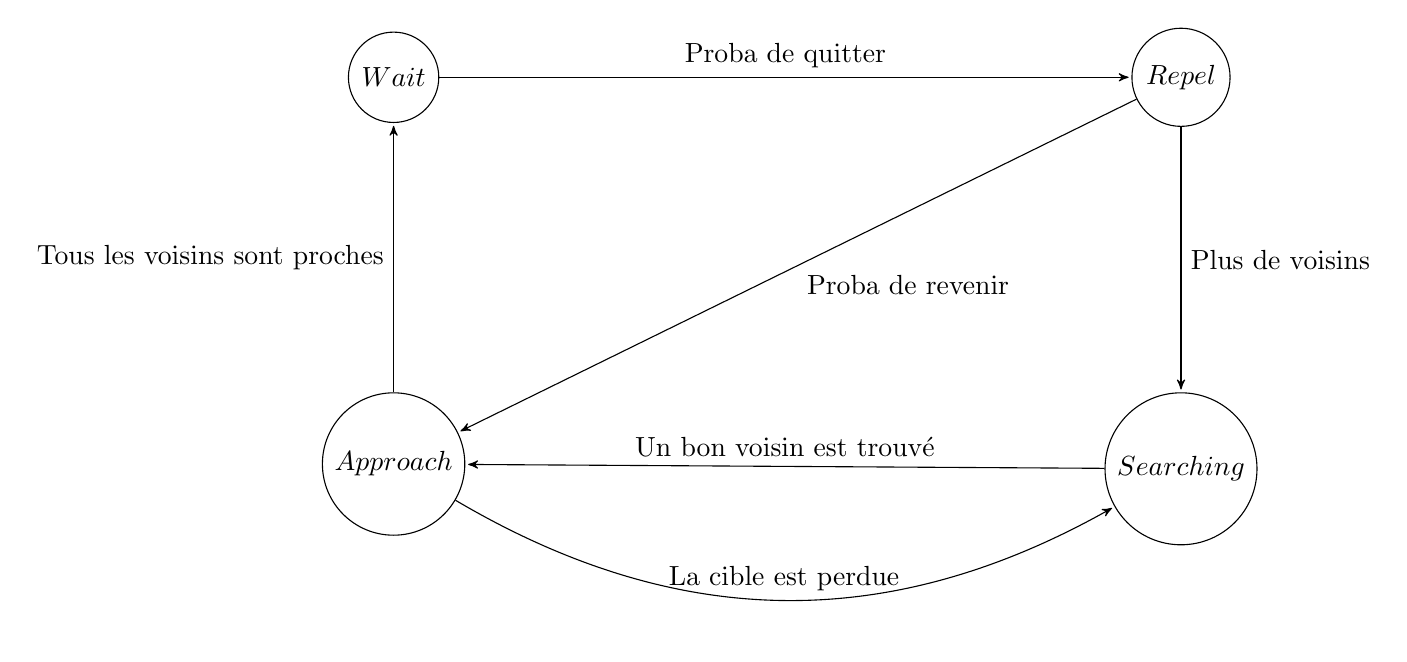
\begin{tikzpicture}[>=stealth',shorten >=1pt,auto,node distance=10cm]
	\node[state] (W)      {$Wait$};
	\node[state] (R) [right of=W]  {$Repel$};
	\node[state] [right of=W,below =4cm] (S)  {$Searching$};
	\node[state] (A)  [below=4cm]{$Approach$};
	
	
	\path[->]
	(A) edge node {Tous les voisins sont proches}(W)
	(S) edge [anchor=south]node {Un bon voisin est trouvé}(A)
	(A) edge [bend right]node {La cible est perdue} (S)
	(W) edge  [sloped] node {Proba de quitter} (R)
	(R) edge   node {Plus de voisins} (S)
	(R) edge node {Proba de revenir} (A)
	;
	\end{tikzpicture}
	\caption{Agrégation probabiliste}
\end{figure}
\newpage
\subsection{Résultats}
\subsubsection{Agrégation naïve}
\begin{figure}[h]
	\begin{minipage}[c]{.46\linewidth}
		\centering
		\includegraphics[width=1.1\linewidth]{../../script_results/Agregation_naive_loss}
		\caption{Nombre de robots perdu selon la distance maximum d'agrégation}
	\end{minipage}
	\hfill%
	\begin{minipage}[c]{.46\linewidth}
		\centering
		\includegraphics[width=1.1\linewidth]{../../script_results/Resultats_aggreg_naive.jpg}
		\caption{Photo fin d'expérience d'agrégation naïve}
	\end{minipage}
\end{figure}
On remarque ici que plus la distance maximale d'agrégation est grande, mois il y a de robots perdu. En effet, ces derniers ayant une distance plus grande pour entrer en attente, ils ont moins de temps d'approche, et donc moins de chance de se perdre lors de cette approche.\\
Lors des expériences, on remarque que les Kilobots se regroupent en chaines et non en agglomérat. De plus, on remarque que les robots perdus sur les cotés de l'arène ont peut de chance de se sortir de cette bordure. En effet, les robots adjacent les pousse et les empêche de se libérer.
\newpage
\subsubsection{Agrégation probabiliste - Analyse Probabilités}
Cet algorithme se base sur la probabilité d'un robot de quitter son groupe afin de trouver potentiellement un nouveau groupe composé de plus d'individus (et donc plus intéressant). Le paramètre important de cet algorithme est donc le calcul de cette probabilité. Nous avons ici testé trois différentes façon de calculer cette probabilité.
\paragraph{Probabilité constante} Nous utilisons ici la probabilité constante proposé par O.Soyal et E.Sahin comme étant celle pour laquelle ils ont obtenu les meilleurs résultats.
\begin{center}
	$P(x)=0.0001$
\end{center}
\paragraph{Probabilité suivant taille groupe} Afin de permettre aux gros agglomérats de robots de rester ensemble, nous avons défini une probabilité pour un Kilobot de quitter un groupe en fonction du nombre de voisins de celui ci par rapport à une constante définie comme la taille d'un groupe que nous considérons \textit{stable}. Or après expérimentation, nous avons remarqué qu'un robot arrivant au bord d'un agglomérat ne reste pas forcément car connecté que à quelques individus de ce groupe.\\Afin de traiter les deux cas d'appartenance à un groupe (au centre ou sur un bord), nous prenons donc le maximum entre le nombre de voisin du Kilobot et le nombre maximum de voisin du meilleur de ses voisins. Le meilleur de ses voisins étant défini comme le voisin ayant le plus de voisin.
\begin{center}
	$P(x)=\min(1,\frac{v(x)}{TAILLE\_GRAND\_GROUPE})$
\end{center}
avec
\begin{center}
	$v(x)=\max(nombre\_de\_voisin(x),nombre\_de\_voisin(meilleur\_voisin(x))$
\end{center}
\paragraph{Probabilité mixte} Cette probabilité a été trouvé après avoir vu les résultats expérimentaux des deux probabilité précédente. Elle a comme objectif de créer des agglomérats stables en ne permettant pas à un robot de partir s'il appartient à un suffisamment grand groupe, et utilisant la probabilité trouvé par  O.Soyal et E.Sahin. Elle est définie comme :
\begin{center}
	$P(x)=$
	$\begin{cases}
	$0$ &\text{\textit{si v(x) >= TAILLE\_GRAND\_GROUPE }}\\
	$0.0001$ &\text{\textit{sinon}}\\
	\end{cases}$
\end{center}
\begin{figure}[h]
	\begin{minipage}[c]{.46\linewidth}
		\centering
		\includegraphics[width=1.1\linewidth]{../../script_results/Agregation_nombre_clusters.png}
		\caption{Nombre de cluster selon probabilité}
	\end{minipage}
	\hfill%
	\begin{minipage}[c]{.46\linewidth}
		\centering
		\includegraphics[width=1.1\linewidth]{../../script_results/Agregation_taille_cluster.png}
		\caption{Taille moyenne d'un cluster selon la probabilité}
	\end{minipage}
\end{figure}

\begin{figure}[h]
	\centering
	\begin{minipage}[c]{.46\linewidth}
		\centering
		\includegraphics[width=1.1\linewidth]{../../script_results/Agregation_nombre_lost.png}
		\caption{Nombre de robots perdu selon probabilité}
	\end{minipage}
\hfill
	\begin{minipage}[c]{.45\linewidth}
	\centering
	\includegraphics[width=1.1\linewidth]{../../script_results/Resultats_aggregation_proba.jpg}
	\caption{Photo fin expérience agrégation linéaire}
\end{minipage}
\end{figure}
\newpage
%
%On remarque que la probabilité constante et la probabilité mixte, contrairement à ce que l on attendait, donnent les mêmes résultats.
On observe que la probabilité constante, proposée par O.Soysal et E.Sahin, donne un grand nombre de petits groupes. En effet, les agrégats sont formés rapidement et la faible probabilité de partir ne permet pas de la mise en place d'un grand groupe.\\
En revanche, la probabilité suivant la taille du groupe permet de remédier à ce problème. On observe en effet un petit nombre de groupe composée d'un grand nombre d'individu. Un individu dans un petit groupe ayant en effet une forte probabilité d'en sortir. Cependant, cette mesure de probabilité ne domine pas la première, le nombre de robot perdu étant largement supérieur à celle ci.\\
\newpage
\subsubsection{Agrégation probabiliste - Analyse Paramètres}
Afin de remédier aux défauts de la probabilité linéaire suivant la taille d'un grand agrégat, nous avons essayé d'étudier les effets de cette taille TAILLE\_GRAND\_GROUPE, afin de faciliter la création d'un groupe robuste et de minimiser le nombre de robots perdus.\\ \\
\begin{figure}[h]
	\begin{minipage}[c]{.46\linewidth}
		\centering
		\includegraphics[width=1.1\linewidth]{../../script_results/Agregation_nombre_clusters_big_cluster.png}
		\caption{Nombre de cluster selon TAILLE\_GRAND\_GROUPE}
	\end{minipage}
	\hfill%
	\begin{minipage}[c]{.46\linewidth}
		\centering
		\includegraphics[width=1.1\linewidth]{../../script_results/Agregation_taille_big_cluster.png}
		\caption{Taille moyenne d'un cluster selon TAILLE\_GRAND\_GROUPE}
	\end{minipage}
\end{figure}
\begin{figure}[h]
	\centering
	\begin{minipage}[c]{.46\linewidth}
		\centering
		\includegraphics[width=1.1\linewidth]{../../script_results/Agregation_loss_kilobot_big_cluster.png}
		\caption{Nombre de robots perdu selon TAILLE\_GRAND\_GROUPE}
	\end{minipage}
\end{figure}
\\On remarque ici que plus la valeur de TAILLE\_GRAND\_GROUPE est faible, moins les robots se perdent. Cependant, une petite valeur ne donne pas forcement plus de groupes.\\
Une valeur trop haute, en revanche, induit un grand nombre de Kilobot perdu et une taille de groupe plus petite. En effet, un Kilobot a rarement plus de 6~7 voisins autour de lui. La probabilité ne permet donc pas la création d'agrégats stables.
\newpage
\section{mEDEA}
Nous implémentons ici la version Vanilla-EE de l'algorithme mEDEA présenté par J.Montanier, S.Carrignon et N.Bredeche.  \cite{montanier_behavioral_2016} Il permet à un essaim de robot de s'adapter à leur environnement en fonction des contraintes de celui ci.
\subsection{Algorithme}

\begin{figure}[h!]
	\centering
	\begin{lstlisting}
		Initialisation aléatoire du génome;
		while True do
			for i=0 to lifetime do
				if self.genome!=NULL then
					move() //selon le genome
					fitness=calculerFitness()
					transmettre(génome,fitness) //aux voisins accessibles
	
				end if
				genomeQueue=receptionGénome()//traitement des messages
				if genomeQueue!=NULL then
					genomeList.add(genomeQueue)
				end if
			end for
			self.genome=NULL
			if genomeList.size > 0 then
				newGenome=select(genomeList) //selection selon meilleure fitness	
				newGenome=mutation(newGenome) //proba de muter
				self.genome=newGenome
			end if
			genomeList.empty()
		end while
	\end{lstlisting}
	\caption{Vanilla-EE}
\end{figure}
Dans notre cas, l'algorithme est exécuté sur chaque robot et évalue le comportement du robot pendant ses déplacements. Un robot correspond donc aux paramètres du comportement courant.
Un Kilobot ne dispose que de 3 capteurs d'entrée :
\begin{itemize}
	\item[$-$] La luminosité
	\item [$-$]Les messages reçus
	\item [$-$]La distance du message à l'envoyeur(calculé par le Kilobot)\\
\end{itemize}

Il nous a donc fallu créer des capteurs \textit{artificiels} via le transfert d'information entre les Kilobots par message. Notre génome est donc constitué des poids d'un perceptron sans couches cachées. Les entrées sont donc :
\begin{itemize}
	\item[$-$] Une entrée active en permanence comme neurone de biais
	\item [$-$]La moyenne des distances à tous les voisins connus
	\item [$-$]Le nombre de voisin actuel
	\item [$-$]Une entrée binaire associé à la présence ou non du bloc actif\\
\end{itemize}
Il y a deux sorties, correspondantes aux gauche et droit de chaque Kilobot.
Cela nous donne donc un génome de 8 gènes correspondant aux 8 paramètres du perceptron. Chaque paramètre peut prendre 3 valeurs : \{-1,0,1\}.
\begin{figure}[h!]
	\centering
	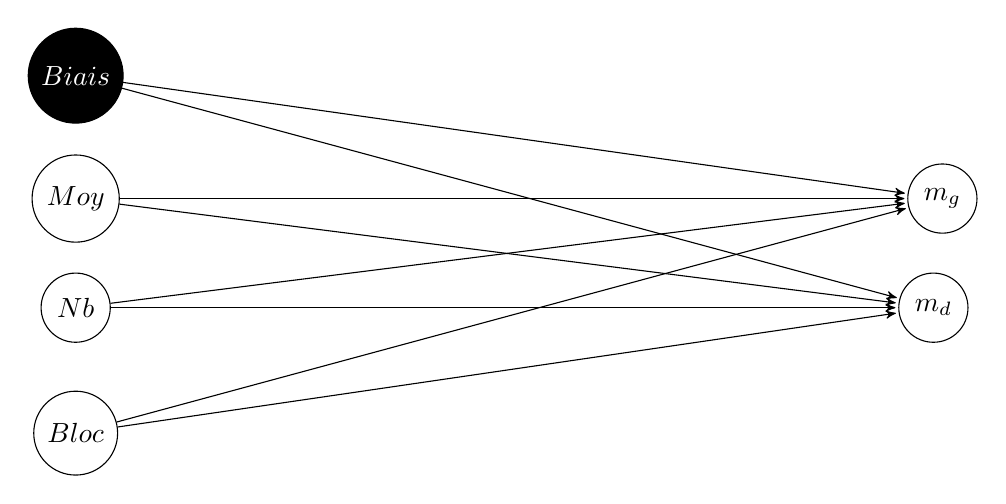
\begin{tikzpicture}[>=stealth',shorten >=1pt,auto,node distance=10cm]
	\node[state,fill=black] (B)      {\textcolor{white}{$Biais$}};
	\node[state] (M) [below =1cm]  {$Moy$};
	\node[state] (S)  [below =2.5cm]  {$Nb$};
	\node[state] (A)  [below=4cm]{$Bloc$};
	\node[state] (MG) [right = of M] {$m_g$};
	\node[state] (MD) [right = of S] {$m_d$};
	
	
	\path[->]
	(B) edge (MG)
	(M) edge  (MG)
	(S) edge  (MG)
	(A) edge  (MG)
	
	(B) edge  (MD)
	(M) edge  (MD)
	(S) edge (MD)
	(A) edge (MD)
	;
	\end{tikzpicture}
	\caption{Controlleur mEDEA}
\end{figure}
\newpage
\paragraph{Fonction d'activation} Notre fonction d'activation permet d'obtenir une sortie dans l'intervalle de vitesse des moteurs :
\begin{center}
$A(x)=\frac{1}{1+e^-x}*(Max\_moteur-Min\_moteur)+Min\_moteur$
\end{center}


\paragraph{Fitness} 
\begin{center}
$F(x)=\sum_{i}  f(x) \qquad \forall{i} \in{0,1,...,evalTime} $

\end{center}
avec
\begin{center}
$f(x)=$
$\begin{cases}
	$1$ &\text{\textit{si Block actif detecte}}\\
	$0$ &\text{\textit{sinon}}\\
\end{cases}$
\end{center}

Notre fitness est ici calculé sur les 40 dernière demi-secondes. Elle est mise à jour à chaque envoie de message du Kilobot vers ses voisins.
\paragraph{Mutation}  La probabilité de mutation est un facteur important de l'algorithme. Un probabilité trop grande peut mener à une population incapable de se stabiliser alors qu'un taux trop bas peut amener à une absence de génome intéressant.
\begin{figure}[h!]
	\centering
	\begin{lstlisting}
	if random() < P_mutation then
		for (i=0;i<len(genome);i++) do
			if random() < 1/len(genome) then
				modif=randint(1,2)
				genome[i]=(genome[i]+modif+1) mod 3 -1
			end if
		end for
	end if
	\end{lstlisting}
	\caption{Mutation}
\end{figure}
\\ Après la décision d'une mutation sur le génome, nous avons décidé de mettre une probabilité fixe de $\frac{1}{nombre de gènes}$ par gène. Cela permettant d'avoir en moyenne un seul gène changé par mutation afin de ne pas avoir un génome changeant drastiquement d'une génération à une autre.
\newpage


\subsection{Résultats}
\subsubsection{Nombre de morts}
\begin{figure}[h]
	\centering
	\begin{minipage}[c]{.46\linewidth}
		\centering
		\includegraphics[width=1.1\linewidth]{../../script_results/mEDEA_1_with_0.png}
		\caption{Nombre de robots mort par génération}
	\end{minipage}
\end{figure}
\subsubsection{Survivabilité d'un génome}
\begin{figure}[h]
	\begin{minipage}[c]{.46\linewidth}
		\centering
		\includegraphics[width=1.1\linewidth]{../../script_results/parent_origine_medea_full.png}
		\caption{Nombre de parent à l'origine des génomes des robots vivant par génération}
	\end{minipage}
	\hfill%
	\begin{minipage}[c]{.46\linewidth}
		\centering
		\includegraphics[width=1.1\linewidth]{../../script_results/parent_origine_medea_zoom.png}
		\caption{Nombre de parent à l'origine des génomes des robots vivant par génération(Zoom)}
	\end{minipage}
\end{figure}

\begin{figure}[h]
	\begin{minipage}[c]{.46\linewidth}
		\centering
		\includegraphics[width=1.1\linewidth]{../../script_results/nombre_genome_different.png}
		\caption{Nombre de génomes différents par génération}
	\end{minipage}
	\hfill%
	\begin{minipage}[c]{.46\linewidth}
		\centering
		\includegraphics[width=1.1\linewidth]{../../script_results/nombre_genome_different_zoom.png}
		\caption{Nombre de génomes différents par génération(Zoom)}
	\end{minipage}
\end{figure}
\newpage
\subsubsection{Comparaison avec expérience témoin}
\newpage
\section{Conclusion}
L’agrégation et la couverture sont des comportements fondamentaux de la robotique en essaim. Les Kilobots offrent un moyen robuste d’étude de ces comportements par leur simplicité et accessibilité, ils permettent une implémentation rapide d’un algorithme distribué tel que mEDEA. Deux types d’agrégation, une couverture ainsi qu’un algorithme d’embodied evolution ont été étudiés.
\\ \\
L’analyse de ces comportements sur robots réels illustre l’avantage d’un simulateur. En effet, le calcul de la distance d’un message reçu peut être défaillant (en raison d’obstructions, de la qualité de la surface utilisée ou d’un défaut matériel) et entraîner une perturbation quant aux résultats obtenus. D’autres facteurs sont à prendre en compte lors de la comparaison de résultats obtenus sur simulateur et en réalité : le bloc actif n’est pas modélisable dans le simulateur et a été remplacé par un Kilobot immobile émettant le signal, il est donc susceptible d’être heurté et déplacé, ce qui n’est pas possible sur le vrai modèle.
\\ \\
Les Kilobots ne possédant pas de capteur de proximité, l’évitement d’obstacle est impossible : les robots viennent à se bloquer entre eux ou contre les murs. Des bandes de LEDs (toujours en phase production à l’ISIR) permettraient aux Kilobots de recevoir des messages des obstacles et ainsi avoir une meilleure perception de l’environnement. Dans le cas de mEDEA, elles apporteraient une entrée supplémentaire au perceptron (et par la même, une solution au manque de capteurs constaté sur les Kilobots). Grâce à ce dispositif, l’étude des algorithmes déployés sera plus précise, ceux-ci contenant majoritairement une marche aléatoire destinée à l’exploration.
\newpage
\section{Bibliographie}

\printbibliography

\end{document}
